\chapter{Architecture}
\label{ch:architecture}

Architecture of Hybrid Graph Model is shown in Fig.\ref{fig:arch}. This can be broadly divided into three segments. First segment consists of information encoders with individual encoders for various levels of data. Second or Middle segment consists of hybrid KG. This graph is constructed, by utilizing vector representations generated by encoders in previous step, and embedding them as, individual piece of information in a node that is relevant. In the Final segment, this hybrid graph is utilized by GCN with attention to extract features of the hybrid KG and final output is a probability distribution of the relations. The author, S. Duan et al.\cite{duan2019hybrid}, proposes to predict the relation between any entity pair $S_{(x_i, y_i)}$ and learn the probability distribution $P(r_i|x_i,y_i;\theta)$ over all relations $r_i \in \mathbb{R}$, where $\theta$ denotes the parameters of the model.

\begin{figure}[h!]
	\centering
	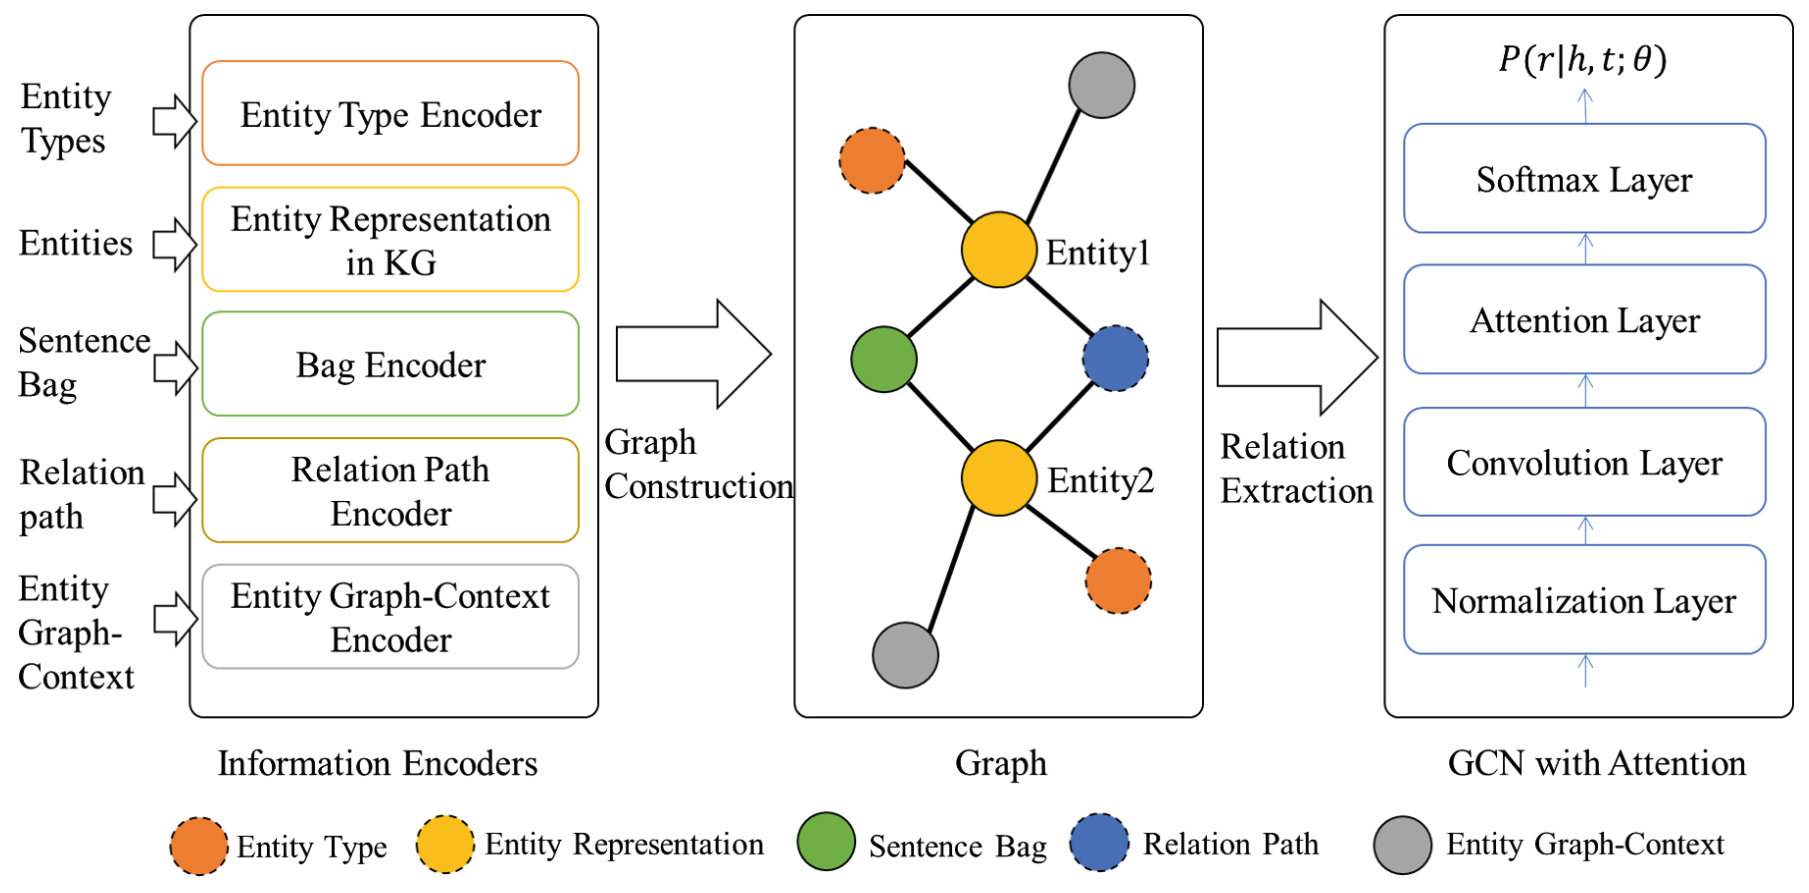
\includegraphics[scale=0.25]{figures/architecture.PNG}
	\caption{The Architecture}
	\label{fig:arch}
\end{figure}

\newpar
Before the process, from a given DS generated data set $D = \{S_{(x_i,y_i)}|,i = 1,2,...\}$, the background information from KG for every entity pair $(x_i, y_i)$ is extracted and stored in a different data set $\mathbb{I} = \{I_{(x_1,y_1)},I_{(x_2,y_2)},...\}$. Label of each instance corresponds to the label of $S_{(x_i, y_i)}$ during the extraction. 




\begin{figure}[h!]
	\centering
	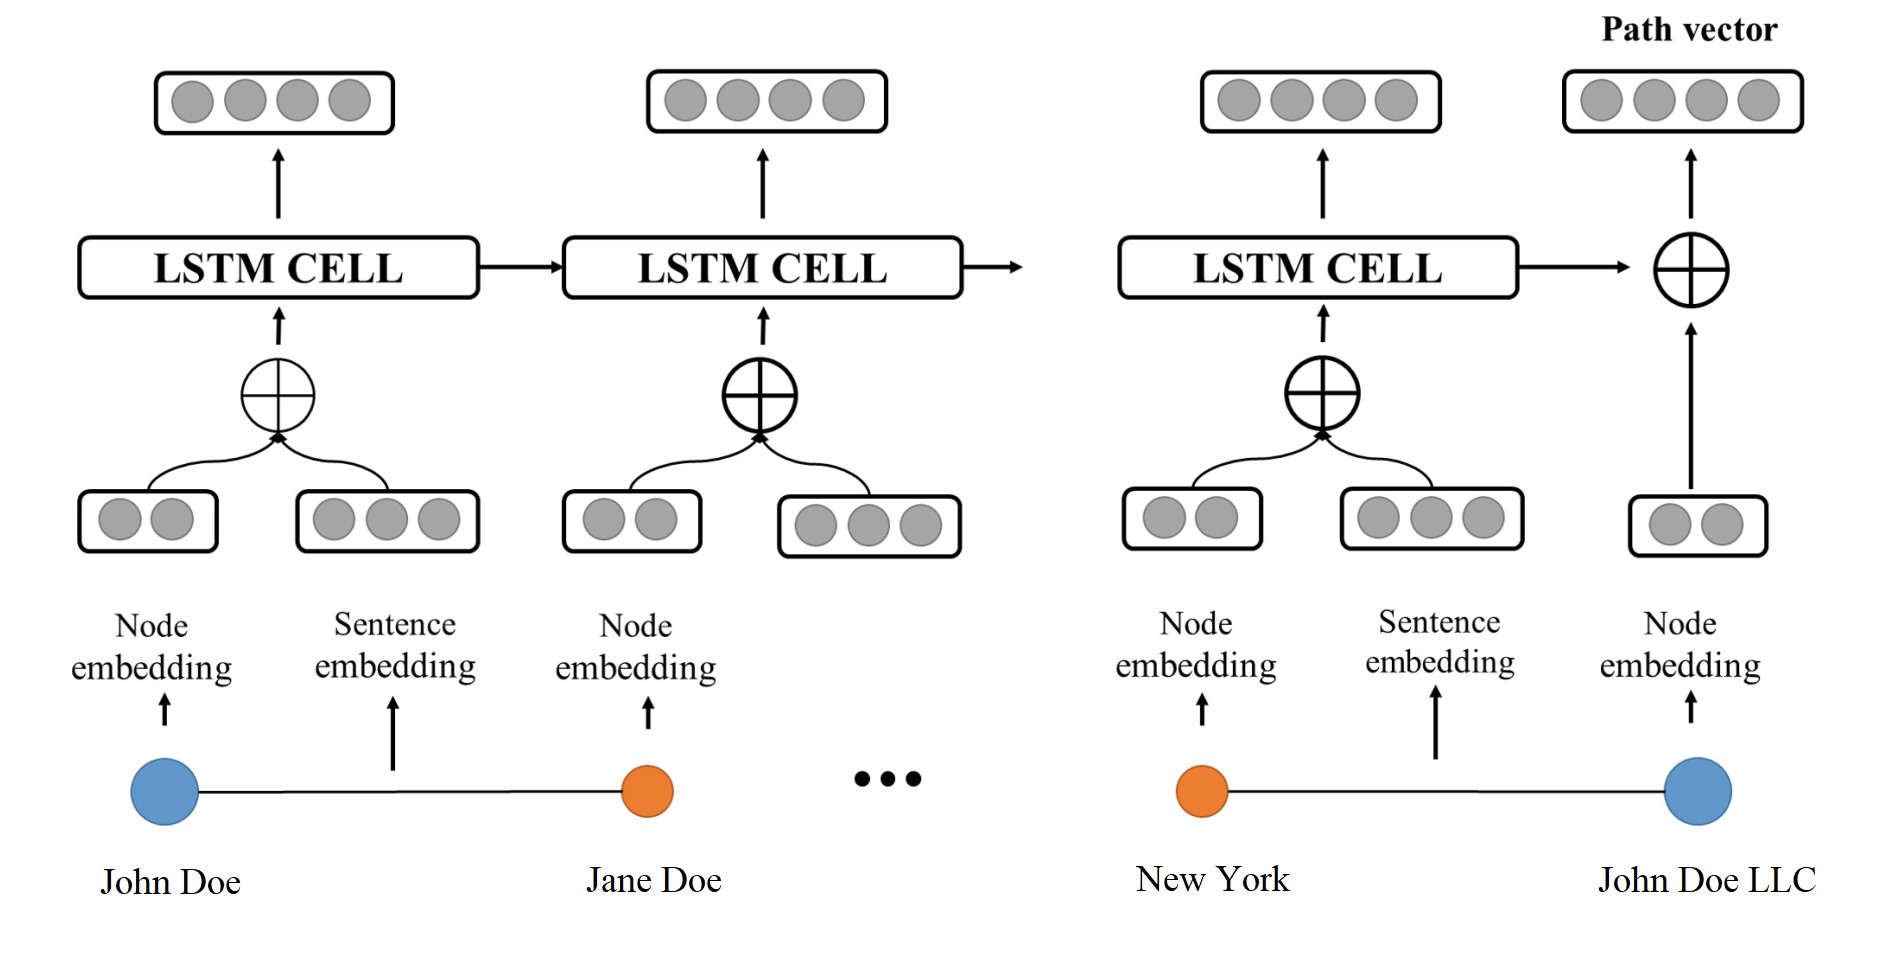
\includegraphics[scale=0.2]{figures/LSTM.PNG}
	\label{fig:lstm}
\end{figure}